% =====================================================================
% Preprint (English) — in silico ASO design for ABCA4 c.161-395G>A
%
% Build:  tectonic docs/preprint_en/preprint_en.tex
% Figures: regenerate with `scripts/run-in-env.sh python pipeline/make_figures.py`
%          They are produced from data/results/, so text and figure cannot diverge.
% =====================================================================
\documentclass[11pt,a4paper]{article}

\usepackage[english]{babel}
\usepackage[utf8]{inputenc}
\usepackage[T1]{fontenc}
\usepackage{geometry}
\geometry{margin=2.5cm}

\usepackage{microtype}          % reduces overfull boxes at the source
\usepackage{graphicx}
\usepackage{booktabs}
\usepackage{array}
\usepackage{amsmath}
\usepackage{amssymb}
\usepackage{bm}
\usepackage{enumitem}
\usepackage{caption}
\usepackage{float}
\usepackage[section]{placeins} % floats never cross a section boundary
\usepackage{needspace}         % keeps a block from being split across pages
\usepackage{xcolor}
\usepackage{fancyhdr}
\usepackage{titlesec}
\usepackage[hidelinks]{hyperref}

\hypersetup{colorlinks=true, linkcolor=blue!50!black, citecolor=blue!50!black,
            urlcolor=blue!50!black,
            pdftitle={An agent-built pipeline for in silico antisense oligonucleotide design},
            pdfauthor={Sergio Mauricio Nunez; Amyra Sanchez}}

% --- typesetting: never let a block break badly -----------------------
\widowpenalty=10000
\clubpenalty=10000
\displaywidowpenalty=10000
\brokenpenalty=10000
\raggedbottom                   % pad the bottom rather than stretch the page
\sloppy                         % prefer loose lines over overfull boxes
\emergencystretch=3em
\setlength{\parskip}{0.45em}
\setlength{\parindent}{0pt}

% Long typewriter identifiers may break at these points instead of overflowing.
\newcommand{\brk}{\discretionary{}{}{}}

\titleformat{\section}{\large\bfseries}{\thesection}{0.8em}{}
\titleformat{\subsection}{\normalsize\bfseries}{\thesubsection}{0.8em}{}
\titlespacing*{\section}{0pt}{1.4em}{0.5em}
\titlespacing*{\subsection}{0pt}{1.0em}{0.35em}

\captionsetup{font=small, labelfont=bf, width=0.94\linewidth}

\pagestyle{fancy}
\fancyhf{}
\fancyhead[L]{\small In silico ASO design for \emph{ABCA4} c.161-395G>A}
\fancyhead[R]{\small Preprint}
\fancyfoot[C]{\thepage}
\renewcommand{\headrulewidth}{0.4pt}

\begin{document}

% =====================================================================
% Cover — hand-built instead of \maketitle, which could not keep the
% author block inside the text width.
% =====================================================================
\thispagestyle{empty}
\begin{center}
  \vspace*{0.6cm}

  {\LARGE\bfseries An agent-built pipeline for in silico\\[0.15em]
   antisense oligonucleotide design,\\[0.25em]
   and what six adversarial reviewers found in it\par}

  \vspace{0.8em}
  {\large A methodological report on \emph{ABCA4} c.161-395G>A\par}

  \vspace{1.6em}
  {\large Sergio Mauricio Nu\~nez\qquad Amyra Sanchez\par}
  \vspace{0.4em}
  {\small \emph{YAIS Lab}\par}
  \vspace{0.2em}
  {\small \href{mailto:mauricio.nunez@yaislab.org}{mauricio.nunez@yaislab.org}\par}

  \vspace{0.9em}
  {\small 2 August 2026 \quad\textbullet\quad Preprint, not peer reviewed\par}
\end{center}

\vspace{0.8em}

\begin{center}
\begin{minipage}{0.88\linewidth}\small\itshape
Implementation, pipeline execution and drafting were carried out by an AI agent
(Claude, Anthropic) under author supervision. Section~\ref{sec:provenance} states
explicitly which decisions were the authors' and which were not.
\end{minipage}
\end{center}

\vspace{1.2em}

\begin{center}
\begin{minipage}{0.92\linewidth}
{\bfseries\large Abstract}\\[0.4em]
\small
The deep-intronic variant \textbf{\emph{ABCA4} c.161-395G>A} activates an aberrant pseudoexon
(PE1b, 91~bp) and was the most prevalent deep-intronic allele in a reported Chinese Stargardt
disease cohort~\cite{wang2025}. No antisense oligonucleotide (ASO) has been published or patented
against it. We report a reproducible seven-module computational pipeline for in silico design of
splice-switching ASO candidates of \textbf{PMO} chemistry~\cite{summerton1997}, built end to end by
an AI agent over six days, and then submitted to a panel of six independent adversarial reviewers.

The pipeline reproduces two results with external anchors. First, the variant installs the
$-2$ consensus adenine of the donor motif over an intact GT dinucleotide
(\texttt{GGG|GTAGGT}~$\rightarrow$~\texttt{GAG|GTAGGT}), a model-free and threshold-free
observation. Second, two independently trained neural predictors~\cite{jaganathan2019,zeng2022}
place their maximum at exactly $+1$ and $-89$ relative to the variant, yielding a predicted
pseudoexon of \textbf{91~bp} that matches the minigene measurement of Wang et al.~\cite{wang2025}
exactly. On an independent published oligo-walk with measured efficacy~\cite{kaltak2023} the same
scoring places the five known-effective AONs at ranks 1, 3, 4, 5 and 6 of 32
($\mathrm{AUC}=0.974$).

We report the adversarial review as a primary result rather than as a limitations paragraph. The
panel returned \emph{reject with invitation to major resubmission} and identified seven critical
issues. Correcting them changed the conclusions: a strand-orientation bug in the melting-temperature
calculation had propagated four modules upstream and generated a finding, a design record and a
published conclusion; a negative control with deliberately wrong tissue reproduced the
``three-predictor agreement'' exactly, showing that agreement to be uninformative; and a claim
repeated across six documents for four days had never been verified against the literature.

\textbf{No candidate has been synthesised or assayed.} We argue that for agent-built research the
adversarial review is not optional quality control but part of the method, and we quantify why.
\end{minipage}
\end{center}

\clearpage

% =====================================================================
\tableofcontents
\clearpage

% =====================================================================
\section{Motivation}

Stargardt disease type~1 is the most common inherited macular dystrophy, caused by biallelic
variants in \emph{ABCA4}. A relevant fraction of pathogenic alleles are not coding variants but
\textbf{deep-intronic variants} that activate cryptic splice sites, leading the spliceosome to
treat an intronic stretch as an exon --- a \emph{pseudoexon} --- and to introduce a premature
termination codon.

Wang et al.~\cite{wang2025} showed by minigene assay that \textbf{c.161-395G>A} activates three
pseudoexons (PE1b 91~bp, PE1c 255~bp, PE1d 265~bp), with 76.4\,\% of the resulting mRNA incorrectly
spliced. They assessed splicing effects with the SpliceAI web lookup and reported only that all
variants exceeded a delta score of 0.2; they did not report cryptic site positions, pseudoexon
coordinates, or a mechanistic account of the base change.

Splice-switching ASOs bind the pre-mRNA by base complementarity and \textbf{sterically block}
access to a splice site without degrading the transcript~\cite{dhuri2020}. No published or patented
ASO targets this variant --- which motivates the work, but also means \textbf{there is no positive
control} with which to validate a design pipeline end to end. Section~\ref{sec:calibration}
describes the partial substitute we used instead.

% =====================================================================
\section{Provenance and division of judgement}
\label{sec:provenance}

We state this before the methods because it conditions how the rest should be read.

The implementation, pipeline execution and drafting were produced by an AI agent. The following
were author decisions, not the agent's:

\begin{itemize}[nosep, leftmargin=1.4em]
  \item \textbf{The chemistry.} PMO was chosen as a scope decision, against the retinal literature
        precedent (2$'$-MOE/PS), and documented with its costs.
  \item \textbf{Commissioning the adversarial review}, on the explicit reasoning that an agent
        cannot audit work it produced.
  \item \textbf{Challenging the agent's assertions.} Three of the highest-impact errors surfaced
        because the authors asked, not because the agent detected them --- as did the fact that PMO
        force-field parameters do exist~\cite{maksudov2023}, after the agent had asserted they did
        not.
\end{itemize}

We consider this disclosure a methodological requirement rather than an acknowledgement.

% =====================================================================
\section{Pipeline}
\label{sec:pipeline}

Seven modules, each with its own reproducible runner and declared limitations
(Table~\ref{tab:modules}, Figure~\ref{fig:funnel}).

\begin{table}[htbp]
\centering
\small
\begin{tabular}{@{}clll@{}}
\toprule
\textbf{\#} & \textbf{Module} & \textbf{Question} & \textbf{Result} \\
\midrule
1  & Sequence         & Where is the variant?              & Coordinate confirmed by two routes~\cite{freeman2018} \\
2  & Oligo-walk       & Which windows?                     & 381 candidates \\
3  & Heuristic filter & Viable oligos?                     & 381 $\rightarrow$ 276 \\
4  & Thermodynamics   & Bind well, reachable?              & 276 $\rightarrow$ 78 \\
5  & Off-target       & Resemble other genes?              & 78 annotated by severity \\
6  & Neural splicing  & Is the false site real?            & Donor $+1$, acceptor $-89$ \\
6b & ASO masking      & Does each patch switch it off?     & 12 abolish the pseudoexon \\
7  & Ranking          & Which to synthesise first?         & Pareto front: 3 \\
\bottomrule
\end{tabular}
\caption{The seven modules and what each one answers. Every row has a regeneration command in the
repository README.}
\label{tab:modules}
\end{table}

\begin{figure}[htbp]
\centering
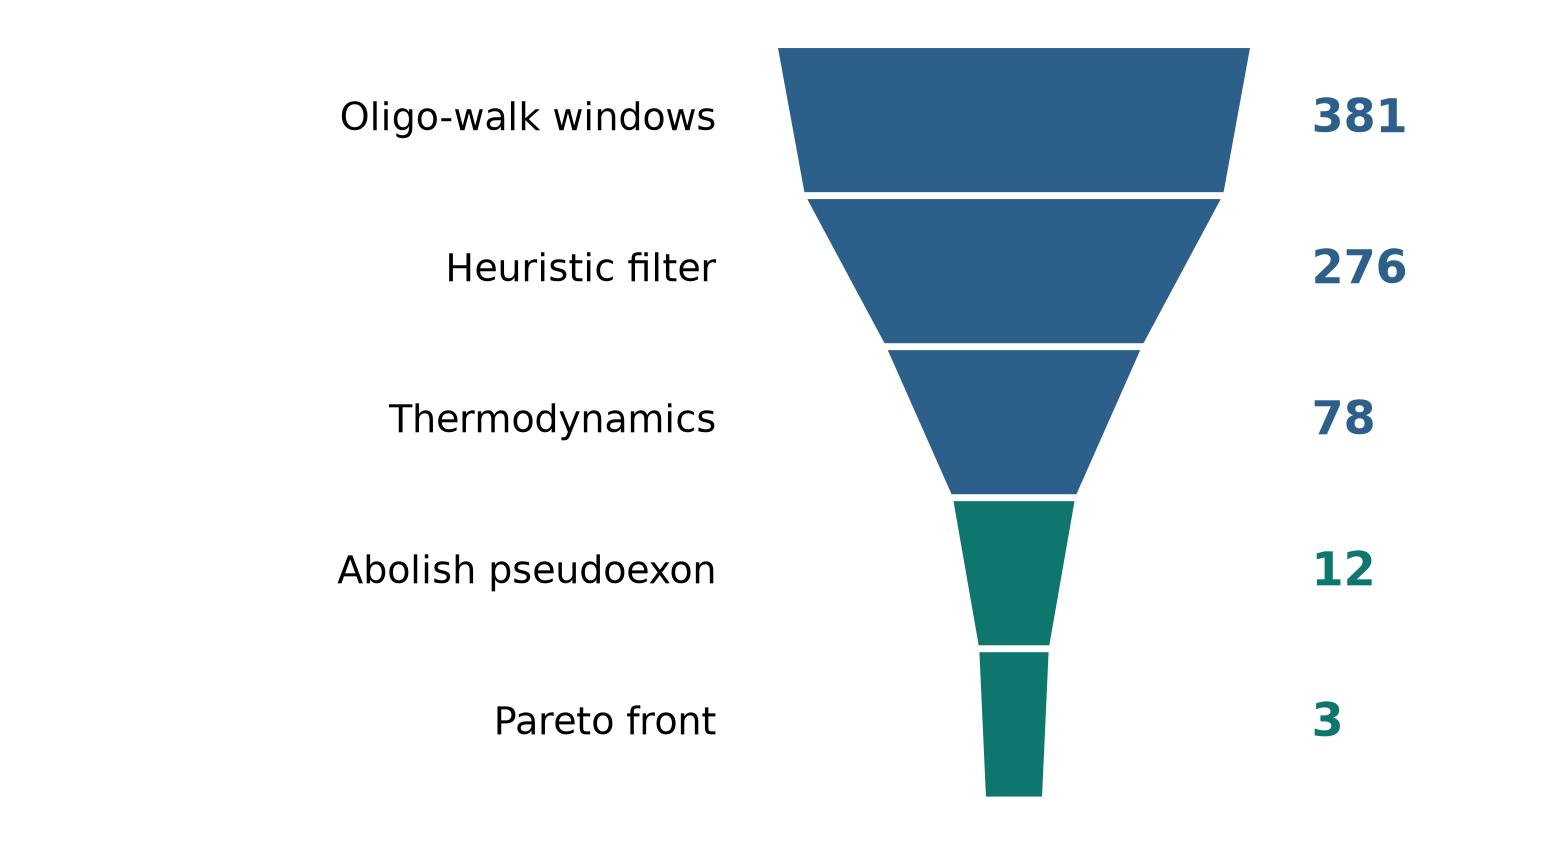
\includegraphics[width=0.9\linewidth]{figs/fig1_funnel.png}
\caption{Candidate funnel with the current numbers. The two green stages are the ones that require
neural inference; everything upstream is sequence arithmetic. The width of each block scales as
$n^{0.42}$ so the last stages remain visible.}
\label{fig:funnel}
\end{figure}

\subsection{Representing an ASO to a splice predictor}
\label{sec:masking}

Splice predictors take a single sequence strand and have no representation of a bound ligand. A PMO
does not cleave or modify the RNA --- it covers it. We therefore replace the ASO window with
\texttt{N}, which the one-hot encoding of both predictor families maps to the null vector: ``no
readable sequence information here''. This is a direct proxy for steric block.

Let $x$ be the mutant pre-mRNA sequence, $c$ a candidate window, and $\mathcal{M}(x,c)$ the same
sequence with every base inside $c$ replaced by \texttt{N}. For a predictor $p$ and a splice site
$s$, write $S_p(\cdot,s)$ for the score it assigns at that position. The quantity the pipeline
actually uses is the \emph{retained fraction of signal}:

\begin{equation}
r_p(c,s) \;=\; \frac{S_p\bigl(\mathcal{M}(x,c),\,s\bigr)}{S_p(x,s)}
\label{eq:retention}
\end{equation}

$r_p = 1$ means the mask changed nothing; $r_p = 0$ means the site disappeared. Expressing the
effect as a ratio rather than a difference is what makes the criterion comparable across predictors
whose score scales differ.

A candidate is judged to \textbf{abolish the pseudoexon} when it switches off \emph{at least one}
of its two borders --- the cryptic donor $d$ at $+1$ or the cryptic acceptor $a$ at $-89$ --- in
\emph{every} predictor:

\begin{equation}
V(c) = \text{abolishes} \iff \forall p \in P:\;
\min_{s \in \{d,\,a\}} r_p(c,s) \;\le\; \tau,
\qquad \tau = 0.25
\label{eq:verdict}
\end{equation}

The disjunction over borders is a biological statement, not a convenience: a pseudoexon needs both
of its borders to be recognised, so removing either one is enough to disassemble it. The threshold
$\tau$ is a declared design choice and is not calibrated against experiment.

Two alternatives were rejected: mutating the window introduces spurious motifs, and excising it
shifts all downstream coordinates. Notably, the predictors' own inference routine already pads with
\texttt{"N"}$\times$5000 on each side, so blocks of \texttt{N} are the operational convention of
these models rather than an invented input.

\subsection{Thermodynamics, and the exact point where the chemistry does not fit}
\label{sec:thermo}

Module~4 estimates the melting temperature of the ASO:RNA duplex with the nearest-neighbour
model~\cite{santalucia1998}, using the RNA/DNA hybrid table of Sugimoto et
al.~\cite{sugimoto1995} as implemented in Biopython~\cite{cock2009}:

\begin{equation}
T_m \;=\; \frac{\Delta H^\circ}{\;\Delta S^\circ + R\,\ln\!\bigl(C_T/x\bigr)\;} \;-\; 273.15
\label{eq:tm}
\end{equation}

with the enthalpy and entropy accumulated over consecutive dinucleotide steps of the sequence
$\bm{s}=s_1s_2\ldots s_n$,

\begin{equation}
\Delta H^\circ = \Delta H^\circ_{\mathrm{init}} + \sum_{i=1}^{n-1} \Delta H^\circ(s_i s_{i+1}),
\qquad
\Delta S^\circ = \Delta S^\circ_{\mathrm{init}} + \sum_{i=1}^{n-1} \Delta S^\circ(s_i s_{i+1}).
\label{eq:nn}
\end{equation}

\needspace{5\baselineskip}
\textbf{The table is asymmetric, and that is what broke.} For a hybrid duplex the parameter set is
indexed by the \textbf{RNA} strand, so $\Delta H^\circ(\mathtt{AG/TT}) \neq
\Delta H^\circ(\mathtt{TT/AG})$. In the tabulated values these differ by more than a factor of two
($-3.96$ vs $-10.38$~kcal\,mol$^{-1}$; $-11.6$ vs $-31.8$~cal\,mol$^{-1}$K$^{-1}$). Passing the ASO
where the RNA target was expected therefore does not produce a small perturbation --- it produces a
different number. Section~\ref{sec:tmbug} reports what that cost.

\textbf{Two biases that do not cancel.} Equation~\ref{eq:tm} assumes a charged backbone, and the
salt correction applied on top of it assumes $\sim$50~mM Na$^+$. A PMO backbone is
neutral~\cite{summerton1997}, and published PMO melting measurements are made near 1.0~M NaCl.
Independently, phosphorodiamidate linkages are reported to \emph{stabilise} the
duplex~\cite{maksudov2023}. Both effects push the estimate in the same direction: the proxy
\textbf{underestimates} the true melting temperature. This is why $T_m$ is now reported as an
annotation and not used as a filter (Section~\ref{sec:recovered}).

\subsection{Off-target}

Module~5 searches each candidate against the human transcriptome with BLAST+~\cite{camacho2009} and
records $L(c)$, the longest perfect contiguous match against any transcript other than
\emph{ABCA4}. Severity is annotated, not gated: for a steric-block chemistry, unlike for an
RNase~H-recruiting gapmer, homology only matters where it lands~\cite{dhuri2020}. Two published
results bound how much this measurement can be trusted: no single sequence feature predicts real
off-target mis-splicing well, and BLAST itself penalises gaps and ignores G:U wobble
pairing~\cite{scharner2020}; and the number of complementary sites grows steeply with the mismatch
tolerance allowed~\cite{yoshida2018}.

\subsection{Ranking: why a Pareto front and not a weighted score}
\label{sec:pareto}

The three ranking dimensions have incomparable units. All are written so that higher is better:

\begin{align}
f_1(c) &= 1 - \frac{1}{|P|}\sum_{p \in P} \min_{s \in \{d,a\}} r_p(c,s)
        && \text{block strength} \label{eq:f1}\\[0.2em]
f_2(c) &= -\,L(c)
        && \text{off-target safety} \label{eq:f2}\\[0.2em]
f_3(c) &= \tfrac{1}{2}\bigl(P_{\mathrm{acc}}(c) + P_{\mathrm{hd}}(c)\bigr)
        && \text{thermodynamic quality} \label{eq:f3}
\end{align}

where $P_{\mathrm{acc}}$ and $P_{\mathrm{hd}}$ are the within-cohort percentiles of target-window
accessibility and of homodimer avoidance, computed with ViennaRNA~\cite{lorenz2011}.

Averaging $f_1$, $f_2$ and $f_3$ into one score requires positing an exchange rate --- how many base
pairs of off-target homology are worth 0.01 of block strength --- that \textbf{no data in this
project supports}, precisely because there is no positive control against which to calibrate it. A
Pareto front requires no such rate. Writing $\bm{f}(c) = (f_1,f_2,f_3)$, candidate $a$
\emph{dominates} $b$ when

\begin{equation}
a \succ b
\iff
\bigl(\forall i:\; f_i(a) \ge f_i(b)\bigr)
\;\wedge\;
\bigl(\exists j:\; f_j(a) > f_j(b)\bigr),
\label{eq:dominance}
\end{equation}

and the front is the set of candidates no one dominates, restricted to those that pass the
eligibility gate $V(c)=\text{abolishes}$ of Equation~\ref{eq:verdict}:

\begin{equation}
\mathcal{F} \;=\; \bigl\{\, a \in E \;:\; \nexists\, b \in E,\; b \succ a \,\bigr\},
\qquad
E = \{\,c : V(c) = \text{abolishes}\,\}.
\label{eq:front}
\end{equation}

It returns a set rather than a winner, which is the honest output.

\needspace{6\baselineskip}
\textbf{The convention we have to declare.} Collapsing accessibility and homodimer avoidance into a
single average in Equation~\ref{eq:f3} \emph{is} an implicit 50/50 weighting --- exactly what this
section claims to avoid. We do it anyway, for a measured rather than aesthetic reason: kept as
separate dimensions, the front grows from 3 to \textbf{11 of the 12} eligible candidates, and a
front that discards almost nothing informs almost nothing. The code reports this number so the
decision stays visible instead of buried.

% =====================================================================
\section{Calibration against an independent oligo-walk}
\label{sec:calibration}

Since no ASO exists for this variant, the pipeline was applied unchanged to a different \emph{ABCA4}
variant that \emph{does} have measured efficacy: c.5461-10T>C in intron~38, for which Kaltak et
al.~\cite{kaltak2023} published a 32-AON walk and reported five as effective, one of which became
the clinical candidate QR-1011. The calibration module is deliberately parallel to the main
pipeline and does not touch it.

Scoring the 32 AONs by the same masking $\Delta$ used in Section~\ref{sec:masking} and asking where
the known-effective ones land gives a Mann--Whitney statistic. With $K$ the known-effective set and
$O$ the rest,

\begin{equation}
U = \sum_{k \in K} \sum_{o \in O}
\Bigl[\mathbf{1}\bigl(\delta_k > \delta_o\bigr) + \tfrac{1}{2}\,\mathbf{1}\bigl(\delta_k = \delta_o\bigr)\Bigr],
\qquad
\mathrm{AUC} = \frac{U}{|K|\,|O|}.
\label{eq:auc}
\end{equation}

The five known-effective AONs occupy ranks \textbf{1, 3, 4, 5 and 6 of 32}, with QR-1011 third:
$\mathrm{AUC} = 0.974$. Repeating the whole calibration with the retina-trained
predictor~\cite{riepe2025} gives the same five ranks and $\mathrm{AUC} = 0.970$, so the separation
is not an artefact of one model. A sensitivity analysis removing the four AONs that cover the
exon~39 acceptor --- where abolishing the site is trivially bad --- leaves 28 AONs and
$\mathrm{AUC} > 0.95$.

\textbf{What this does and does not license.} It shows the scoring is not arbitrary: it discriminates
AONs with measured efficacy on a target it was never tuned for. It does not transfer to
c.161-395G>A, which is a different intron, a different mechanism (pseudoexon inclusion rather than
exon skipping) and a different chemistry.

% =====================================================================
\section{Results with external anchors}

These two do not depend on any metric we defined.

\subsection{The variant installs the donor consensus adenine}

Counting matches against the donor consensus \texttt{MAG|GTRAGT}, the wild-type sequence 1~nt
downstream of the variant reads \texttt{GGG|GTAGGT} and the mutant reads \texttt{GAG|GTAGGT}. The
variant itself supplies the adenine at position $-2$ --- one of the most conserved positions of the
donor consensus --- over an intact GT dinucleotide, with purines at $+3$ and $+5$. This requires no
model, no threshold and no predictor.

\subsection{The predicted pseudoexon size matches an independent experiment}

SpliceAI~\cite{jaganathan2019} local inference over a 10~kb window predicts a cryptic donor gained
at $+1$ ($0.194 \rightarrow 0.560$) and a cryptic acceptor at $-89$ ($0.061 \rightarrow 0.271$). The
implied pseudoexon is \textbf{91~bp}, identical to the PE1b measured by minigene in Wang et
al.~\cite{wang2025} --- computational prediction and in vitro measurement converging by fully
independent routes.

Pangolin~\cite{zeng2022}, a different architecture trained by a different group, places its maximum
at \emph{exactly} the same two positions, with neighbouring positions at $\sim$1e$-$5. A deliberate
attempt to break this result during adversarial review failed.

\textbf{What does not follow.} SpliceAI does not explain PE1c or PE1d: their implied acceptors score
0.016 and 0.042, far below any usable threshold. The model accounts for one of three reported
pseudoexons, and we state this rather than omit it.

\subsection{Which windows switch the pseudoexon off}

Applying Equations~\ref{eq:retention} and~\ref{eq:verdict} to the 78 candidates that reach
Module~6b gives Figure~\ref{fig:masking}. Two distinct mechanisms appear, and they are not
interchangeable.

\begin{figure}[htbp]
\centering
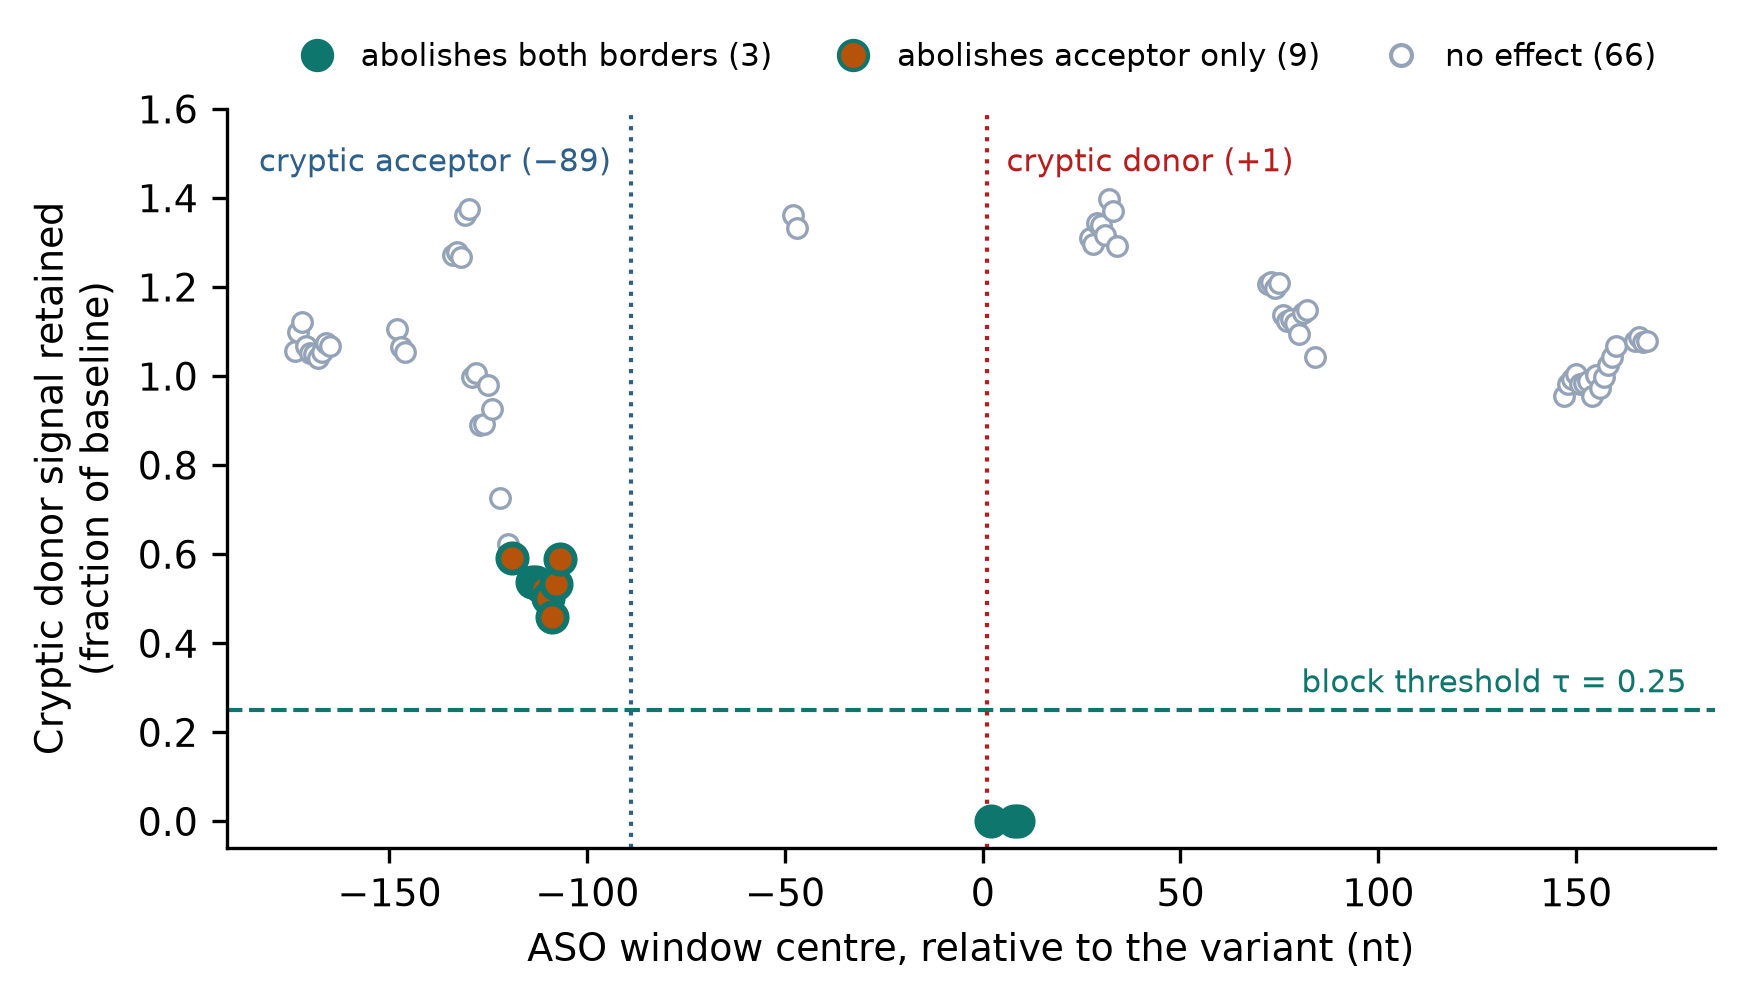
\includegraphics[width=\linewidth]{figs/fig2_masking.png}
\caption{Effect of masking each candidate window on the cryptic donor signal, as a fraction of the
unmasked baseline (Equation~\ref{eq:retention}). Windows covering the donor at $+1$ drive it to
zero. Nine candidates centred near $-110$ abolish the \emph{acceptor} without covering the donor,
and are visible here only as a partial drop in donor signal --- their acceptor retention is what
Equation~\ref{eq:verdict} evaluates. The dashed line is the declared threshold $\tau = 0.25$.}
\label{fig:masking}
\end{figure}

% =====================================================================
\section{The adversarial review as a result}
\label{sec:review}

Six independent reviewers --- splicing biology, statistics, reproducibility, ASO therapeutics, code
integrity, and a hostile red team --- were given a dossier of every claim with its evidence level
and regeneration command, plus explicit rules of engagement requiring that each objection cite a
file, line or number.

The verdict was \emph{reject with invitation to major resubmission}. Seven critical issues were
raised. Four were independently verified before acceptance. Figure~\ref{fig:impact} summarises what
changed; the subsections give the mechanism of each.

\begin{figure}[htbp]
\centering
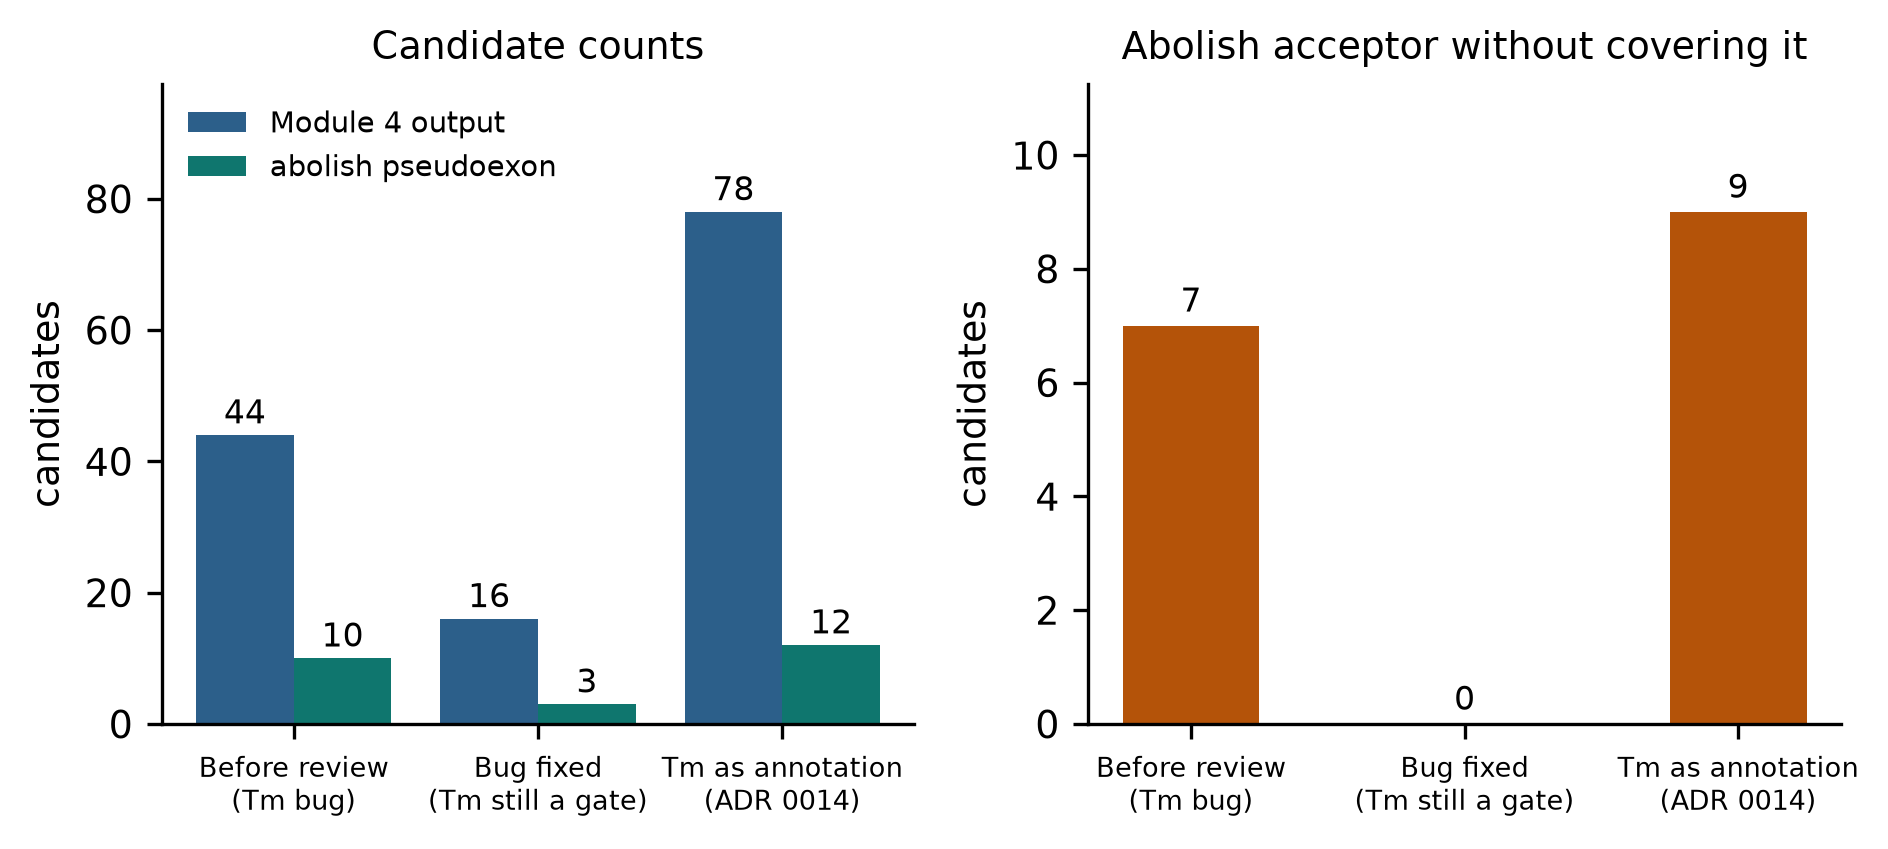
\includegraphics[width=\linewidth]{figs/fig3_review_impact.png}
\caption{What the review changed. \textbf{Left:} candidates surviving Module~4 and, of those, how
many abolish the pseudoexon. \textbf{Right:} candidates that abolish the cryptic acceptor without
covering it --- the observation that had motivated the project's verdict criterion. It existed
before the review for the wrong reason (a bug), vanished entirely when the bug was fixed, and
reappeared on solid ground once $T_m$ stopped being used as a filter.}
\label{fig:impact}
\end{figure}

\subsection{A Module 4 bug that travelled four modules upstream}
\label{sec:tmbug}

\texttt{Bio.SeqUtils.\brk MeltingTemp.\brk Tm\_NN} with the \texttt{R\_DNA\_NN1} table documents
that the argument must be the \textbf{RNA} strand; the code passed the ASO. As shown in
Section~\ref{sec:thermo}, the table is asymmetric, so the order changes the number.

Correcting it moved the Module~4 funnel from \textbf{44 to 16} candidates, with only 6 in common.
More consequentially, the seven candidates that abolished the acceptor \emph{without covering it}
--- the observation that had motivated the project's verdict criterion, its own design record, and a
published conclusion about predictor agreement --- \textbf{did not survive}. A defect in the
cheapest module had generated a finding four modules downstream: not a wrong number, but a wrong
claim about biology.

\subsection{A wrong-tissue control that dissolved an argument}

The project had reported that three independently trained predictors, one of them
retina-specific~\cite{riepe2025}, selected the same exact candidate set, and presented this as
cross-validation. The panel proposed the missing control: run a model trained on \emph{deliberately}
the wrong tissue --- the GTEx weight set released alongside Retina-SpliceAI, which excludes neural
retina (Figure~\ref{fig:tissue}).

\textbf{The wrong tissue selects the retina model's candidates one for one}: both return the same
11 of 78, candidate for candidate, not merely the same count. The agreement therefore reflects
shared architecture and shared training annotations, not tissue-robust biology. The control cost six
minutes of CPU and had been available since the weights were installed; nobody in the project had
run it, because nobody was looking for a way to refute their own argument.

\begin{figure}[htbp]
\centering
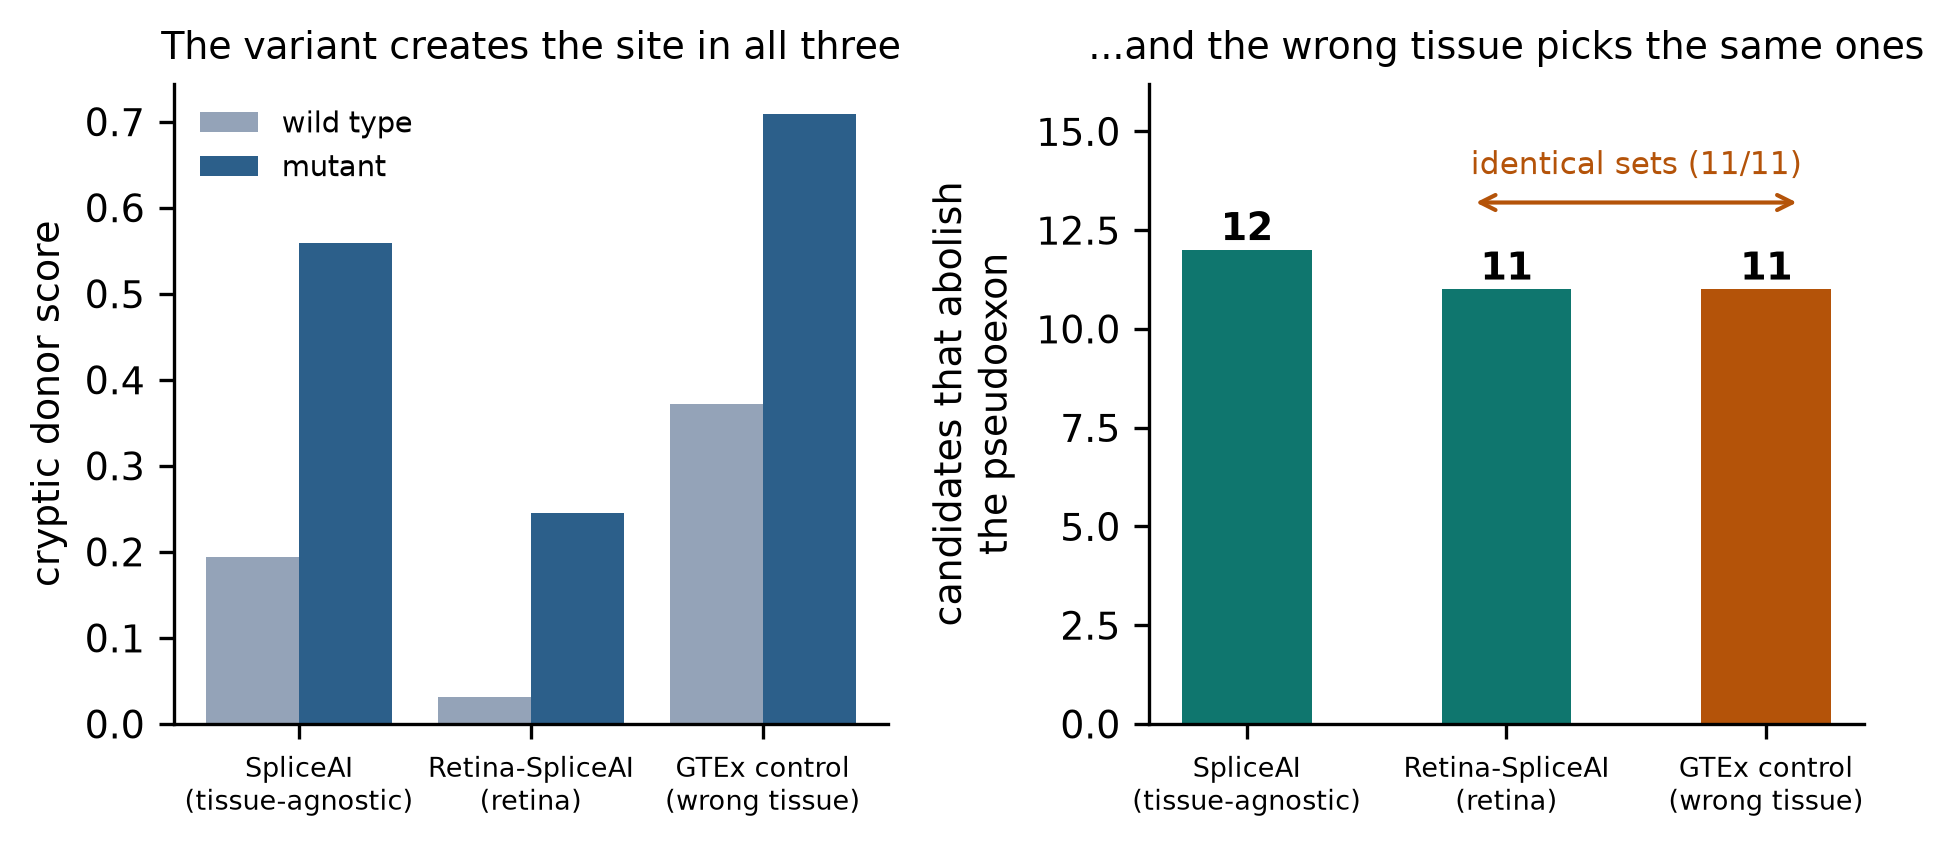
\includegraphics[width=\linewidth]{figs/fig4_tissue_control.png}
\caption{The negative control. \textbf{Left:} all three weight sets --- tissue-agnostic,
retina-trained, and a GTEx model that deliberately excludes neural retina --- agree that the variant
creates the cryptic donor, though they disagree on its absolute strength. \textbf{Right:} the
retina model and the wrong-tissue model select \emph{identical} candidate sets (11 of 78); the
tissue-agnostic model differs by one. Since the wrong tissue reproduces the result, agreement
between them cannot be evidence of tissue-robust biology.}
\label{fig:tissue}
\end{figure}

\subsection{A claim repeated for four days without verification}

The assertion that no nearest-neighbour thermodynamic parameters exist for PMO propagated through
six documents from a single unverified inference. Checking it found: the claim is essentially
correct for PMO, but the NN model \emph{is} documented as applicable to uncharged oligomers;
parameters \emph{do} exist for 2$'$-MOE/PS~\cite{park2025}, the chemistry of the actual retinal
literature; and PMO force-field parameters \emph{do} exist~\cite{maksudov2023}. Further, the
experimental evidence shows phosphorodiamidate linkages \emph{stabilise} the duplex, so the proxy
\textbf{underestimates} the true melting temperature --- a bias in the same direction as the
inapplicable salt correction, so the two accumulate rather than cancel.

\subsection{A correction that recovered what the filter had hidden}
\label{sec:recovered}

Because the melting-temperature threshold could not be interpreted for this chemistry, it was
converted from a filter into an annotation --- following a precedent the project had already set for
off-target severity. The funnel went from 16 to \textbf{78} candidates.

The acceptor-only candidates \textbf{reappeared}: nine of them, with proxy melting temperatures of
36.5--40.1\,$^\circ$C, all below the discarded threshold. The mechanism was real; the buggy
calculation had admitted them for the wrong reason and the corrected gate had hidden them entirely.
The final Pareto front returns to the same three candidates as the original analysis, now by a
defensible route.

\subsection{A misattributed citation, found while assembling this bibliography}
\label{sec:misattribution}

While compiling the reference list for this preprint, the source of the minigene measurement was
checked against Crossref and PubMed Central for the first time. The DOI and PMC identifier the
project had recorded were correct; the author name was not. The paper is
\textbf{Wang et al.}~\cite{wang2025} --- there is no author named Peng on it. The attribution had
been wrong in 19 places across the repository and in 15 vault documents, for five days, and had
already been read by the six reviewers without any of them flagging it.

We report it because it is the same failure mode as the other three: a claim that was never checked
against its source, repeated until repetition made it look verified. It is also the cheapest of the
four to have caught --- one API call --- and the last one found.

% =====================================================================
\section{The candidates that survive}
\label{sec:candidates}

Twelve of the 78 candidates abolish the pseudoexon under Equation~\ref{eq:verdict} in both
predictors. Three are non-dominated under Equation~\ref{eq:dominance} (Table~\ref{tab:front}).

\begin{table}[htbp]
\centering
\small
\begin{tabular}{@{}lccccc@{}}
\toprule
\textbf{Candidate} & \textbf{Window} & \textbf{Borders} & $f_1$ & $f_2$ & $f_3$ \\
 & (rel. to variant) & abolished & block & off-target & thermo \\
\midrule
\texttt{cand\_5992} & $-8$ to $+12$    & donor + acceptor & 1.000 & $-15$ & \phantom{0}8.45 \\
\texttt{cand\_5998} & $-2$ to $+18$    & donor + acceptor & 1.000 & $-16$ & \phantom{0}9.75 \\
\texttt{cand\_5882} & $-118$ to $-98$  & acceptor only    & 0.994 & $-15$ & 70.75 \\
\bottomrule
\end{tabular}
\caption{The Pareto front. Each candidate is 20~nt. $f_2$ is the negated longest perfect contiguous
match against another transcript (Equation~\ref{eq:f2}), so $-15$ is safer than $-16$. Note the
trade-off the front exposes: the two strongest blockers are the two \emph{worst} on
physicochemical properties, and the acceptor-only candidate is the reverse. Nothing in this project
determines which trade-off is preferable --- that is a human decision, which is why the pipeline
returns three rows and not one.}
\label{tab:front}
\end{table}

\textbf{No candidate has been synthesised, transfected or assayed.} Table~\ref{tab:front} is a
synthesis order of priority, conditional on someone deciding to synthesise anything at all.

% =====================================================================
\section{What this pipeline does not do}

Stated with every result and not omissible when communicating it.

\begin{itemize}[nosep, leftmargin=1.4em]
  \item \textbf{No experimental validation.} No ASO synthesised or assayed.
  \item \textbf{The masking proxy does not measure efficacy.} Equation~\ref{eq:retention} is binary
        and total: it assumes 100\,\% occupancy and perfect block. Necessary, not sufficient.
  \item \textbf{PMO thermodynamics are a proxy of another chemistry}, now correctly oriented but
        still not PMO, and biased in a known direction (Section~\ref{sec:thermo}).
  \item \textbf{Off-target severity thresholds are uncalibrated} design choices.
  \item \textbf{Predictor agreement is not independent} and, per the tissue control, largely
        uninformative.
  \item \textbf{The pipeline is blind to splice-site displacement}: it scores four fixed offsets
        and discards the rest of the profile.
  \item \textbf{The threshold $\tau = 0.25$ in Equation~\ref{eq:verdict} is a declared convention},
        not a measured cut-off.
\end{itemize}

% =====================================================================
\section{Discussion}

The scientific contribution of this work is modest and bounded: a mechanistic account of one
pseudoexon, computationally confirmed, plus a reproducible pipeline that produces a shortlist no
one has tested.

The methodological contribution is, we think, larger. An AI agent produced a system with real
engineering discipline --- 224 tests, three documented environments, provenance files, archived
pre-correction results --- and simultaneously produced conclusions that did not survive contact with
adversarial review. Crucially, \textbf{the failures were not arithmetic}. Six reviewers found no
calculation error. They were failures of framing: which metric to define, which control not to run,
which claim to repeat without checking --- and, as Section~\ref{sec:misattribution} shows, which
citation never to open.

That asymmetry is the finding we would emphasise. Agent-built research is likely to be strong where
the work is mechanical and weak where it requires deciding what would refute you. Adversarial review
is therefore not quality control appended at the end; for this mode of work it is part of the
method.

% =====================================================================
\section{Availability}
\label{sec:availability}

Code, results and regeneration commands: \url{https://github.com/smnunez404/bio-oligonucleotidos}
(MIT licence; generated data CC BY 4.0). Every number cited here has a regeneration command in the
repository README, and the figures in this preprint are generated from
\texttt{data/results/} by a versioned script, so text and figure cannot diverge. The adversarial
review report and the claims dossier are maintained in the project's documentation vault and are
available on request.

\section*{Acknowledgements}
\addcontentsline{toc}{section}{Acknowledgements}

We thank the authors of SpliceAI (Illumina), Pangolin (Zeng \& Li), Retina-SpliceAI
(Riepe et al., CMBI/Radboud UMC) and ViennaRNA for making their work openly available, and Wang
et al.\ and Kaltak et al.\ for the experimental measurements that made external anchoring possible.

% =====================================================================
\clearpage
\addcontentsline{toc}{section}{References}
\begin{thebibliography}{99}
\small

\bibitem{wang2025}
Wang Y, Wang P, Yi Z, Ouyang J, Jiang Y, Li S, Jia X, Xiao X, Hejtmancik JF, Sun W, Zhang Q.
\emph{ABCA4 deep intronic variants contributed to nearly half of unsolved Stargardt cases with a
milder phenotype.} Invest Ophthalmol Vis Sci. 2025;66(1):65.
\href{https://doi.org/10.1167/iovs.66.1.65}{doi:10.1167/iovs.66.1.65}

\bibitem{kaltak2023}
Kaltak M, de Bruijn P, Piccolo D, Lee SE, Dulla K, Hoogenboezem T, Beumer W, Webster AR,
Collin RWJ, Cheetham ME, Platenburg G, Swildens J.
\emph{Antisense oligonucleotide therapy corrects splicing in the common Stargardt disease type
1-causing variant ABCA4 c.5461-10T>C.} Mol Ther Nucleic Acids. 2023;31:674--688.
\href{https://doi.org/10.1016/j.omtn.2023.02.020}{doi:10.1016/j.omtn.2023.02.020}

\bibitem{jaganathan2019}
Jaganathan K, Kyriazopoulou Panagiotopoulou S, McRae JF, et al.
\emph{Predicting splicing from primary sequence with deep learning.}
Cell. 2019;176(3):535--548.e24.
\href{https://doi.org/10.1016/j.cell.2018.12.015}{doi:10.1016/j.cell.2018.12.015}

\bibitem{zeng2022}
Zeng T, Li YI. \emph{Predicting RNA splicing from DNA sequence using Pangolin.}
Genome Biol. 2022;23(1):103.
\href{https://doi.org/10.1186/s13059-022-02664-4}{doi:10.1186/s13059-022-02664-4}

\bibitem{riepe2025}
Riepe TV, de Bruijn SE, Roosing S, Cremers FPM, 't Hoen PAC.
\emph{Deep learning-based prediction of tissue-specific splice sites in the human neural retina.}
bioRxiv, posted 13 February 2025.
\href{https://doi.org/10.1101/2025.02.10.637427}{doi:10.1101/2025.02.10.637427}

\bibitem{sugimoto1995}
Sugimoto N, Nakano S, Katoh M, Matsumura A, Nakamuta H, Ohmichi T, Yoneyama M, Sasaki M.
\emph{Thermodynamic parameters to predict stability of RNA/DNA hybrid duplexes.}
Biochemistry. 1995;34(35):11211--11216.
\href{https://doi.org/10.1021/bi00035a029}{doi:10.1021/bi00035a029}

\bibitem{santalucia1998}
SantaLucia J Jr. \emph{A unified view of polymer, dumbbell, and oligonucleotide DNA
nearest-neighbor thermodynamics.} Proc Natl Acad Sci USA. 1998;95(4):1460--1465.
\href{https://doi.org/10.1073/pnas.95.4.1460}{doi:10.1073/pnas.95.4.1460}

\bibitem{summerton1997}
Summerton J, Weller D. \emph{Morpholino antisense oligomers: design, preparation, and properties.}
Antisense Nucleic Acid Drug Dev. 1997;7(3):187--195.
\href{https://doi.org/10.1089/oli.1.1997.7.187}{doi:10.1089/oli.1.1997.7.187}

\bibitem{maksudov2023}
Maksudov F, Kliuchnikov E, Pierson D, et al.
\emph{Therapeutic phosphorodiamidate morpholino oligonucleotides: physical properties, solution
structures, and folding thermodynamics.} Mol Ther Nucleic Acids. 2023;31:631--647.
\href{https://doi.org/10.1016/j.omtn.2023.02.007}{doi:10.1016/j.omtn.2023.02.007}

\bibitem{park2025}
Park SW, Lee J, Park JW, et al. \emph{Thermodynamic parameter estimation for modified
oligonucleotides using molecular dynamics simulations.} J Phys Chem B. 2025.
\href{https://doi.org/10.1021/acs.jpcb.4c08344}{doi:10.1021/acs.jpcb.4c08344}

\bibitem{lorenz2011}
Lorenz R, Bernhart SH, H\"oner zu Siederdissen C, Tafer H, Flamm C, Stadler PF, Hofacker IL.
\emph{ViennaRNA Package 2.0.} Algorithms Mol Biol. 2011;6:26.
\href{https://doi.org/10.1186/1748-7188-6-26}{doi:10.1186/1748-7188-6-26}

\bibitem{camacho2009}
Camacho C, Coulouris G, Avagyan V, Ma N, Papadopoulos J, Bealer K, Madden TL.
\emph{BLAST+: architecture and applications.} BMC Bioinformatics. 2009;10:421.
\href{https://doi.org/10.1186/1471-2105-10-421}{doi:10.1186/1471-2105-10-421}

\bibitem{cock2009}
Cock PJA, Antao T, Chang JT, et al. \emph{Biopython: freely available Python tools for computational
molecular biology and bioinformatics.} Bioinformatics. 2009;25(11):1422--1423.
\href{https://doi.org/10.1093/bioinformatics/btp163}{doi:10.1093/bioinformatics/btp163}

\bibitem{freeman2018}
Freeman PJ, Hart RK, Gretton LJ, Brookes AJ, Dalgleish R.
\emph{VariantValidator: accurate validation, mapping, and formatting of sequence variation
descriptions.} Hum Mutat. 2018;39(1):61--68.
\href{https://doi.org/10.1002/humu.23348}{doi:10.1002/humu.23348}

\bibitem{scharner2020}
Scharner J, Ma WK, Zhang Q, Lin KT, Rigo F, Bennett CF, Krainer AR.
\emph{Hybridization-mediated off-target effects of splice-switching antisense oligonucleotides.}
Nucleic Acids Res. 2020;48(2):802--816.
\href{https://doi.org/10.1093/nar/gkz1132}{doi:10.1093/nar/gkz1132}

\bibitem{dhuri2020}
Dhuri K, Bechtold C, Quijano E, Pham H, Gupta A, Vikram A, Bahal R.
\emph{Antisense oligonucleotides: an emerging area in drug discovery and development.}
J Clin Med. 2020;9(6):2004.
\href{https://doi.org/10.3390/jcm9062004}{doi:10.3390/jcm9062004}

\bibitem{yoshida2018}
Yoshida T, Naito Y, Sasaki K, Uchida E, Sato Y, Naito M, Kawanishi T, Obika S, Inoue T.
\emph{Estimated number of off-target candidate sites for antisense oligonucleotides in human mRNA
sequences.} Genes Cells. 2018;23(6):448--455.
\href{https://doi.org/10.1111/gtc.12587}{doi:10.1111/gtc.12587}

\bibitem{sullivan2024}
Sullivan PJ, Quinn JMW, Wu W, Pinese M, Cowley MJ.
\emph{SpliceVarDB: a comprehensive database of experimentally validated human splicing variants.}
Am J Hum Genet. 2024;111(10):2164--2175.
\href{https://doi.org/10.1016/j.ajhg.2024.08.002}{doi:10.1016/j.ajhg.2024.08.002}

\end{thebibliography}

\end{document}
